% =====================================================================================
%  How Much Full Attention Does Long Context Need?  --  IE624 pre-project report (short)
%  Build:  tectonic -X compile main.tex      (or: latexmk -xelatex main.tex)
%  The longer draft with extra figures is report_long.tex.
% =====================================================================================
\documentclass[10pt,a4paper]{article}
\usepackage{iereport}
\title{How Much Full Attention Does Long Context Need?}
\author{Punit Ranawat \and Tanish Kharbanda \and Rajdeep Agarwal}
\date{November 2026}
\begin{document}

\begin{titlepage}
\newgeometry{top=1.0in,bottom=1.0in,left=1.25in,right=1.25in}
\centering

\includegraphics[width=2.6cm]{figures/iitb_logo.pdf}\par
\vspace{0.45cm}
{\large Indian Institute of Technology Bombay\par}
\vspace{0.15cm}
{\normalsize IE624: Generative and Agentic AI\par}
\vspace{2.6cm}
\rule{\textwidth}{4pt}\par
\vspace{0.42cm}
{\fontsize{22}{27}\selectfont\bfseries How Much Full Attention Does\\[3pt] Long Context Need?\par}
\vspace{0.32cm}
{\large A Controlled Study of Hybrid Full/Linear Attention\\ in Language Models Trained from Scratch\par}
\vspace{0.38cm}
\rule{\textwidth}{1pt}\par
\vspace{0.5cm}
{\large Pre-Project Report\par}
\vspace{2.2cm}
\begin{tabular}{c@{\hspace{2.6em}}c@{\hspace{2.6em}}c}
\textbf{Punit Ranawat} & \textbf{Tanish Kharbanda} & \textbf{Rajdeep Agarwal} \\
24B2715 & 24B2231 & 24B2455 \\
\end{tabular}\par
\vfill
{\small Code and data: \url{https://github.com/mr-entr0py/hybrid-attention-longcontext}\par}
\vspace{0.2cm}
{\small 14 November 2026\par}
\restoregeometry
\end{titlepage}

\setcounter{page}{1}
\begin{center}
{\fontsize{15}{19}\selectfont\bfseries How Much Full Attention Does Long Context Need?\par}
\vspace{0.25cm}
{Punit Ranawat \quad Tanish Kharbanda \quad Rajdeep Agarwal\par}
{\small IE624: Generative and Agentic AI, IIT Bombay\par}
\end{center}
\vspace{0.1cm}
\begin{center}{\large\bfseries Abstract}\end{center}
\vspace{-0.25cm}
\begin{list}{}{\setlength{\leftmargin}{0.5in}\setlength{\rightmargin}{0.5in}}\item[]
Long-context language models, and the agents built on them, pay for memory with attention. Full
attention keeps a key--value cache that grows with every token, while linear attention compresses the
past into a fixed-size state. Most recent long-context architectures are hybrids that keep a few full
attention layers among many linear ones, but their ratios are often inherited or chosen without a published sweep.
We study the choice directly. We train 12-layer language models from scratch that differ \emph{only} in the number $k$ of
full-attention layers, with the remaining $12-k$ layers using Gated DeltaNet. Parameters, data and recipe are held fixed. We will evaluate
retrieval, multi-hop and aggregation at 1K--32K tokens and measure inference cost on one implementation.
This report presents the motivation, theory and pre-registered design. It also presents the completed
engineering and validation work on a single 16\,GB RTX~5080, including the reproduction of published
recall results. No main-study model has been trained yet, so we make no claims about the hypotheses.
\end{list}

% =====================================================================================
\section{Introduction}
For a long-running agent the context window is working memory. What the model can recover from early
in its context bounds what it can reason about later, and the cost of holding that context bounds how
long it can run and how many users it can serve. Both are set by the token-mixing layer. Full attention
\citep{vaswani2017attention} can retrieve any earlier token exactly, but its key--value (KV) cache grows
linearly with context and its prefill cost quadratically. Linear-attention and state-space layers
\citep{katharopoulos2020transformers,dao2024transformers,yang2025gated} keep a state of fixed size. That
makes them cheap, but it is a lossy memory, and both theory and experiment show such models struggle with exact
recall and copying \citep{arora2023zoology,jelassi2024repeat,wen2024rnns}.

Hybrids such as Jamba \citep{lieber2024jamba}, Nemotron-H \citep{nvidia2025nemotronh}, MiniMax-01
\citep{minimax2025minimax01}, Qwen3-Next \citep{qwen2025qwen3next} and Kimi Linear \citep{kimi2025linear}
keep one full-attention layer in every four to eight. They thereby answer, implicitly, the question \emph{how
much full attention is enough?} The answers are rarely tested. Nemotron-H, for instance, sets about
8\% attention layers ``as suggested by prior work'' \citep{waleffe2024empirical}, and neither MiniMax-01 nor
Qwen3-Next publishes the sweep behind its ratio. We therefore ask, under controlled conditions,
\emph{how retrieval, multi-hop composition and aggregation over long inputs change as the number of
full-attention layers varies with everything else fixed, and what each layer costs at inference}.

The question concerns LLMs generally, but answering it causally requires many models that differ in
exactly one factor, with several seeds each. Converting large pretrained checkpoints cannot provide this.
We therefore train models of 28--49M parameters from scratch. The cost mechanisms, KV-cache growth and
fixed-state interference, have the same form at any scale, and controlled small-model studies have been a
main source of evidence on them \citep{arora2023zoology,waleffe2024empirical}. Their capability consequences
may change with scale, so every conclusion will be scoped to the scale studied.

% =====================================================================================
\section{Background}
\paragraph{Full attention.} A head with dimension $d_h$ outputs
$\vect{o}_t=\sum_{i\le t}\softmax_i(\vect{q}_t^{\T}\vect{k}_i/\sqrt{d_h})\,\vect{v}_i$, a content-weighted
average over \emph{all} earlier values. A query that matches one key sharply retrieves its value almost
exactly, however distant. Prefill costs $O(T^2d)$ and decoding must read a cache of
\begin{equation}\label{eq:kv}
  M_{\Full}(T)=2\cdot T\cdot d\cdot 2\ \text{bytes}=4Td\ \text{bytes}
\end{equation}
per layer in 16-bit precision (heads spanning the full width, no key--value sharing), so decode bandwidth and the number of concurrent sequences both scale with $T$.

\paragraph{Linear attention as associative memory.} Replacing the exponential kernel by a feature-map
product \citep{katharopoulos2020transformers} turns attention into a recurrence on a matrix state:
\begin{equation}\label{eq:lin}
  S_t=S_{t-1}+\vect{v}_t\phi(\vect{k}_t)^{\T},\qquad \vect{o}_t=S_t\phi(\vect{q}_t).
\end{equation}
Memory is constant in $T$. However, a read $S\vect{q}=\sum_i\vect{v}_i(\phi(\vect{k}_i)^{\T}\phi(\vect{q}))$ returns one
stored value cleanly only if the other stored keys are orthogonal to the query, and a $d_k$-dimensional state holds at most $d_k$ orthogonal keys. Beyond that, stored
associations interfere \citep{schlag2021linear}.

\paragraph{Delta rule and Gated DeltaNet.} The delta rule takes one gradient step of size $\beta_t$ on
$\tfrac12\lVert S\vect{k}_t-\vect{v}_t\rVert^2$, which replaces a fraction $\beta_t$ of the value currently retrieved by $\vect{k}_t$ instead
of adding to it (a full overwrite when $\beta_t=1$ and keys have unit norm) \citep{schlag2021linear,yang2024deltanet}. Gated DeltaNet \citep{yang2025gated} adds a
data-dependent decay $\alpha_t\in(0,1)$:
\begin{equation}\label{eq:gdn}
  S_t=S_{t-1}\,\alpha_t\big(I-\beta_t\vect{k}_t\vect{k}_t^{\T}\big)+\beta_t\vect{v}_t\vect{k}_t^{\T},
  \qquad \vect{o}_t=S_t\vect{q}_t ,
\end{equation}
with L2-normalised $\vect{q},\vect{k}$ (each projection passes through a short causal convolution) and an output gate. It can both forget and edit
selectively. It is the linear layer of Qwen3-Next and has mature kernels that run on our GPU
\citep{fla2024}, so we adopt it as our linear mixer.

\paragraph{Cost of a hybrid.} With $k$ of $L$ layers using full attention and a fixed linear state
$S_{\Lin}$ per layer, the inference state of a length-$T$ sequence is
\begin{equation}\label{eq:state}
  M(k,T)=k\cdot 4Td+(L-k)\,S_{\Lin}\ \text{bytes}.
\end{equation}
In our D384 model $S_{\Lin}=110{,}592$\,B while one attention layer adds 1,536\,B per token. A single
attention layer therefore outweighs a whole linear layer after 72 tokens, and at 32K the 12-layer model
needs 1.3\,MiB with $k=0$ but 576\,MiB with $k=12$. The open question is what each of these layers buys.

% =====================================================================================
\section{What is known}
Controlled ratio sweeps
\citep{waleffe2024empirical,dao2024transformers,bae2025hybrid,wang2025systematic,kimi2025linear} agree
on language-modelling loss. Once roughly 5--10\% of layers use attention, loss is flat or U-shaped in the
ratio, and an all-attention model is often worse than the best hybrid. Recall behaves differently. In the
only controlled sweep that tabulates it \citep{wang2025systematic}, RULER recall averaged over four linear
mechanisms rises from 0.256 (no attention) to 0.397 (one layer in four), while language-modelling metrics
stay within 0.47--0.48. That recall is averaged over tasks and measured at a single, short (2K--4K) training length. The only experiment that
crosses the amount of full attention with length, from Nemotron-Flash \citep{fu2025nemotronflash},
finds that keeping one full-attention layer instead of three leaves short-context recall unchanged but lowers retrieval on RULER's hardest single-needle task at 32K
from 0.69 to 0.32. That experiment uses sliding-window layers and continued pretraining.
Positional encoding is a known confound, since removing it from the attention layers of hybrids can
improve long-context retrieval \citep{qiao2026nope}. No study we located combines a full $0\to L$ sweep
under matched parameters, data and recipe, with seeds; results by task family and by length, all within
the training length; and costs measured on one implementation. We expect to \emph{reproduce} flat
loss and saturating recall. What is new is the controlled, length- and task-resolved recall curve and
its relation to cost.

% =====================================================================================
\section{Research questions and hypotheses}
Each model has $L=12$ layers with mixers $\vect{a}\in\{\Full,\Lin\}^{12}$, and $k=\sum_l\mathbb{1}[a_l=\Full]$.
For task family $f$ and length $T$ let $S_f(k,T)$ be the per-seed accuracy, and define the recovered
fraction of the all-attention advantage
\begin{equation}\label{eq:rec}
  R_f(k,T)=\frac{S_f(k,T)-S_f(0,T)}{S_f(12,T)-S_f(0,T)} .
\end{equation}
We ask how performance depends on $k$ (\textbf{RQ-A}), on the placement of the attention layers
(\textbf{RQ-B}), and on the task (\textbf{RQ-C}), and how it relates to measured cost (\textbf{RQ-D}). The
hypotheses below, with their tests, were fixed before any training. The central one is
\textbf{H1}: three attention layers recover more than 80\% of the advantage on retrieval at 16K--32K (using only
lengths where the all-attention reference passes a pre-registered adequacy check, with an 8K fallback labelled as such). Since
$S(3)-0.2\,S(0)-0.8\,S(12)=G\,(R-0.8)$ with gap $G=S(12)-S(0)>0$, it is tested as a one-sided paired $t$-test of
$L_3=S(3)-0.2\,S(0)-0.8\,S(12)>0$. The other hypotheses are as follows.
\textbf{H1$_{\min}$}: one layer suffices.
\textbf{H2}: diminishing returns in $k$ (descriptive).
\textbf{H3}: multi-hop needs more attention than retrieval, $R_{\text{ret}}(3)-R_{\text{hop}}(3)>0$.
\textbf{H4}: placement matters at fixed $k$.
\textbf{H5}: the gap $S(12)-S(0)$ grows with $\log T$.
\textbf{H6}: hybrids reach a cost--capability region that neither extreme reaches (descriptive).
H1, H1$_{\min}$, H3 and H5 form a Holm-corrected family \citep{holm1979simple}.

% =====================================================================================
\section{Study design}
\begin{figure}[t]
\centering
\begin{tikzpicture}[font=\footnotesize]
  % ---- (a) one block
  \begin{scope}[node distance=2.6mm]
    \node[box,minimum width=2.75cm] (emb) {token embedding $E$ (tied)};
    \node[box,minimum width=2.75cm,above=4.5mm of emb] (n1) {RMSNorm};
    \node[box,fill=fillg,line width=0.8pt,draw=black,minimum width=2.75cm,minimum height=6mm,above=of n1] (mix) {\textbf{mixer} $a_l\in\{\Full,\Lin\}$};
    \node[circle,draw=black!70,inner sep=0.4pt,above=2.2mm of mix] (p1) {\scriptsize$+$};
    \node[box,minimum width=2.75cm,above=2.2mm of p1] (n2) {RMSNorm};
    \node[box,minimum width=2.75cm,above=of n2] (mlp) {SwiGLU MLP};
    \node[circle,draw=black!70,inner sep=0.4pt,above=2.2mm of mlp] (p2) {\scriptsize$+$};
    \node[box,minimum width=2.75cm,above=4.5mm of p2] (out) {RMSNorm $\to$ logits};
    \foreach \u/\v in {emb/n1,n1/mix,mix/p1,p1/n2,n2/mlp,mlp/p2,p2/out} {\draw[->,black!70] (\u) -- (\v);}
    \coordinate (r1) at ($(n1.south)+(0,-1.5mm)$);
    \draw[->,black!70,rounded corners=1pt] (r1) -| ($(mix.west)+(-2.6mm,0)$) |- (p1.west);
    \coordinate (r2) at ($(p1.north)+(0,1.0mm)$);
    \draw[->,black!70,rounded corners=1pt] (r2) -| ($(mlp.west)+(-2.6mm,0)$) |- (p2.west);
    \node[draw=black!50,dashed,rounded corners=1pt,inner sep=2mm,fit=(n1)(p2)] (blk) {};
    \node[anchor=west,font=\small] at (blk.east) {$\times12$};
    \node[lab,above=1.5mm of out] {(a) one block};
  \end{scope}
  % ---- (b) the two mixers
  \begin{scope}[xshift=3.75cm]
    \node[box,draw=fullc,line width=0.6pt,text width=3.85cm,align=left,anchor=north west,font=\scriptsize] (F) at (0,5.55) {%
      {\footnotesize\textbf{$\Full$: full softmax attention}}\\[1.5pt]
      64-dim heads (6 heads at D384)\\
      per-head QK-RMSNorm\\
      RoPE, $\theta=5\cdot10^5$, reset per doc.\\
      head-wise sigmoid output gate\\[1.5pt]
      \textit{state: KV cache, $4d$ bytes per token}};
    \node[box,draw=fullc!60,line width=0.6pt,fill=linc!35,text width=3.85cm,align=left,anchor=north west,font=\scriptsize] (L) at ($(F.south west)+(0,-0.35)$) {%
      {\footnotesize\textbf{$\Lin$: Gated DeltaNet}}\\[1.5pt]
      $S_t=S_{t-1}\alpha_t(I-\beta_t\vect{k}_t\vect{k}_t^{\T})+\beta_t\vect{v}_t\vect{k}_t^{\T}$\\
      $d_k{=}64$, $d_v{=}128$, conv width 4\\
      output normalisation and gate\\[1.5pt]
      \textit{state: fixed, 108\,KiB per layer (D384)}};
    \node[lab,anchor=south] at ($(F.north)+(0,0.12)$) {(b) the two token mixers};
  \end{scope}
  % ---- (c) configurations
  \begin{scope}[xshift=9.05cm,yshift=0.25cm]
    \def\cw{0.275}\def\ch{0.36}
    \foreach \k/\pos [count=\row from 0] in {0/{},1/{6},2/{3,9},3/{2,6,10},6/{1,3,5,7,9,11},12/{0,1,2,3,4,5,6,7,8,9,10,11}} {
      \pgfmathsetmacro{\yy}{4.75-\row*0.56}
      \foreach \l in {0,...,11} {\fill[linc] (\l*\cw+0.015,\yy) rectangle ++(\cw-0.03,\ch);}
      \foreach \l in \pos {\fill[fullc] (\l*\cw+0.015,\yy) rectangle ++(\cw-0.03,\ch);}
      \node[anchor=east,font=\scriptsize] at (-0.04,\yy+0.19) {$k=\k$};
    }
    \foreach \l in {0,3,6,9,11} {\node[font=\tiny,text=ink2] at (\l*\cw+0.15,1.6) {\l};}
    \node[lab] at (1.8,1.3) {layer (input $\to$ output)};
    \node[lab,anchor=south] at (1.8,5.25) {(c) configurations C$k$};
    \fill[fullc] (0.15,0.72) rectangle ++(0.25,0.2); \node[lab,anchor=west] at (0.45,0.82) {full ($\Full$)};
    \fill[linc] (1.85,0.72) rectangle ++(0.25,0.2); \node[lab,anchor=west] at (2.15,0.82) {GDN ($\Lin$)};
  \end{scope}
\end{tikzpicture}
\caption{The model family. (a) All models share 12 pre-norm blocks. (b) The only per-layer difference is the
token mixer. (c) Configuration C$k$ places $k$ full-attention layers at evenly spaced positions. Across
$k$, non-embedding parameter counts differ by at most 0.14\% (21.31M vs.\ 21.28M at D384; 41.01M vs.\ 40.97M at D512).}
\label{fig:arch}
\end{figure}

\paragraph{Models.} Every model is a stack of 12 pre-norm blocks (RMSNorm, mixer, residual, RMSNorm,
SwiGLU MLP, residual) with tied embeddings (\cref{fig:arch}). The full mixer is multi-head attention
with 64-dimensional heads, QK-normalisation \citep{henry2020qknorm}, RoPE with base $5\times10^5$
\citep{su2024roformer,dubey2024llama3} reset at each document, and a head-wise output gate
\citep{qiu2025gated}. The linear mixer is Gated DeltaNet (\cref{eq:gdn}) from \code{fla}~0.6.0. Two
scales are prepared, D384 (27.6M parameters) and D512 (49.4M), and a pilot rule picks one. The main sweep is
$k\in\{0,1,3,12\}$, with $k\in\{2,6\}$ and early/late placement as a second tier. Three controls
address known confounds: the same short convolution added to attention \citep{olsson2022induction},
attention without positional encoding \citep{kazemnejad2023nope}, and a single-head linear layer with roughly three to four times the state.

\paragraph{Data and training.} We train on FineWeb-Edu \citep{penedo2024fineweb} and PG19 books
\citep{rae2020compressive}, pinned to exact revisions, with a 16K-entry BPE tokenizer that splits digits.
Books are essential: only about 2\% of FineWeb-Edu tokens lie in documents of 32K tokens or more,
against 97\% for PG19. Every configuration follows one recipe. Stage~A trains at 4K tokens on 0.6--0.8B tokens.
Stage~B extends to 32K tokens, so every evaluation length lies inside the training length. A short,
identical task-exposure fine-tune on synthetic tasks follows, with disjoint words and templates, because models of
this size are expected to score at the floor zero-shot (Wang et al.\ found recall insignificant even at 340M). Training uses AdamW \citep{loshchilov2019adamw},
bf16 and a learning rate chosen on held-out loss, never on task metrics.

\paragraph{Evaluation and cost.} Natural-language long-context benchmarks score at the floor at this
scale \citep{hsieh2024ruler}. We therefore use cloze tasks scored by teacher-forced exact match, built in
token space to exactly $T$ tokens with filler from held-out documents. \emph{Retrieval} hides facts among
distractors and loads up to 1,024 associations, probing the capacity of a fixed state. \emph{Multi-hop} follows
shuffled chains of up to four references. \emph{Aggregation} compares word frequencies across the input. Each
cell has 200--300 contexts at $T\in\{1\text{K},\dots,32\text{K}\}$. Costs are reported analytically (\cref{eq:state},
FLOPs, bytes moved) and as measured prefill and decode latency under CUDA graphs on an idle GPU.

\paragraph{Statistics and integrity.} The unit of inference is the training run: four to five seeds per
configuration, paired across $k$ through a shared data order and initialisation. ``Falsified'' requires
a competent all-attention reference and robustness to longer fine-tuning and a doubled Stage~B. Every
threshold is hashed before its experiment, a failed check is recorded as \emph{not passed as registered}
rather than relabelled, and every decision is logged with the evidence that would reopen it. In keeping
with the course theme, the work is agent-assisted. LLM agents carried out literature reading, two
independent adversarial reviews of the design, module construction and verification, with role
separation so that no agent verified its own code.

% =====================================================================================
\section{Completed engineering and validation}
\paragraph{Environment.} All work runs on one NVIDIA RTX~5080 (Blackwell, 16\,GB) with 62\,GB RAM, PyTorch~2.11
(CUDA~12.8), Triton~3.6 and \code{flash-linear-attention}~0.6.0. Official Mamba kernels and external
FlashAttention wheels are unavailable for this stack, and attention uses PyTorch's built-in
FlashAttention-2 path. Each process is capped at about 7\,GiB, and 32K-token steps use activation
checkpointing (3.1\,GiB peak; 6.0\,GiB is the highest peak of any stage). The GPU also drives the display, whose
7-second driver watchdog is active, and seven watchdog faults (Xid~8) occurred during early runs. Our longest
32K kernel takes 25\,ms, so long kernels are not the cause; a pre-registered soak test will localise it.

\paragraph{Verification.} Of the 451 tests in 20 families of infrastructure checks with pre-fixed
thresholds, 447 pass and 4 are skipped. Our all-attention model matches the reference \code{Qwen3ForCausalLM} to a relative
logit error of $7\times10^{-7}$, and our all-GDN model matches the reference \code{fla} model to $4.6\times10^{-4}$.
Inference state equals \cref{eq:state} to the byte, and cached decoding reproduces a full forward pass in fp32.
Independent verifiers found and fixed real defects: an unshuffled multi-hop control solvable by a positional heuristic, replay data
crossing document boundaries, and about 25.7K held-out documents duplicating training text. Six sub-items, for
example a precision bound and one D512 throughput measurement, missed their literal criteria without isolating a
code defect, so the gate is recorded as \emph{not passed as registered}, with a named residual risk for each.

\begin{table}[t]
\centering\small
\caption{Reproductions of published results. Pass criteria were fixed before each run.}
\label{tab:repro}
\begin{tabularx}{\textwidth}{@{}>{\raggedright\arraybackslash}p{4.3cm} X l@{}}
\toprule
Reproduction & Result & Verdict\\
\midrule
MQAR, Zoology code \citep{arora2023zoology} & overall accuracy: attention $\ge$0.9997; GDN 0.989 ($d$=128), 0.994 ($d$=256) & pass\\
Our mixers in Zoology's harness & within 0.0004 of the reference in all cells & pass\\
MQAR below ceiling ($d$=64, 3 seeds) & hardest cell, $d$=64/128/256: 0.30$\to$0.93$\to$0.96; ours vs.\ reference at $d$=64: $-0.018$ & pass\\
LAMBADA, GDN-340M \citep{wang2025systematic} & 0.3435 vs.\ published 0.348 & pass\\
LAMBADA, Pythia-160M/70M \citep{biderman2023pythia} & fp32 0.354/0.227; fp16 0.330/0.185 (published 0.328/0.185) & not as registered\\
Exactness vs.\ independent references & 1/5 pass; 3 uncalibrated tolerances; 1 generator flaw (fixed, re-check pending) & not as registered\\
\bottomrule
\end{tabularx}
\end{table}

\begin{figure}[t]
  \centering
  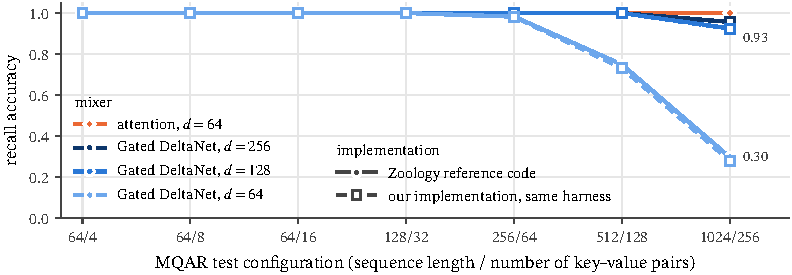
\includegraphics[width=\textwidth]{figures/fig_mqar.pdf}
  \caption{Reproduction of the recall--state trade-off on MQAR \citep{arora2023zoology}. Solid lines are Zoology's code
  and dashed lines are our layers in the same harness. Gated DeltaNet's fixed state saturates as key--value pairs
  grow (most visibly at width 64, three seeds) while attention stays at 1.0. Our layers show no large deviation from the reference.}
  \label{fig:mqar}
\end{figure}

\paragraph{Reproductions.} We reproduced published results with the original code first and then with our
components substituted (\cref{tab:repro}). On multi-query associative recall (MQAR), the canonical
demonstration that fixed-state recall degrades with load \citep{arora2023zoology}, our layers match the
reference within 0.0004 overall. At width 64 they are within $-0.018$ of it, although this pre-registered test can
exclude only a handicap larger than about 0.11 (\cref{fig:mqar}). The recall--state trade-off our study builds on is
therefore present and measurable in our stack. On LAMBADA \citep{paperno2016lambada} our scorer reproduces the public GDN
checkpoint. The Pythia anchors failed as registered: three independent scorers agree item for item, and
the published numbers turn out to come from half-precision weights, which we reproduce to within 0.0014.
Three of the exactness failures are floating-point rounding against uncalibrated bounds. The fourth exposed
value-prefix collisions in 7 of 39,800 queries; the generator has been fixed and the items regenerated, but the
pre-registered re-check has not yet run.

\begin{figure}[t]
  \centering
  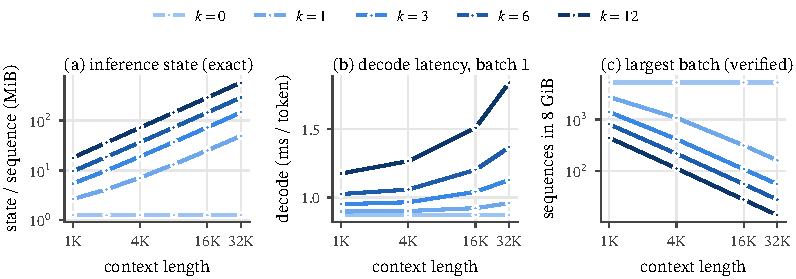
\includegraphics[width=\textwidth]{figures/fig_cost2.pdf}
  \caption{Cost side of the trade-off at D384, measured on untrained weights (session 1 of 2). (a) Exact state per
  sequence, from \cref{eq:state} and verified on the device. (b) Per-token decode latency, minimum of $\ge$30
  CUDA-graph replays. (c) Largest batch whose state and decoding activations fit in an 8\,GiB budget.}
  \label{fig:cost}
\end{figure}

\paragraph{Preliminary measurements.} Speed does not depend on trained weights, so it was measured
early. These are engineering numbers, not findings. Training throughput at 4K tokens is nearly independent of $k$,
at 127--138K tokens/s for D384. At 32K it falls from 107K ($k=0$) to 78K ($k=12$) tokens/s, so compute per token is not matched across
configurations. A complete D384 run takes about two GPU-hours. At inference (\cref{fig:cost}) the all-linear model
decodes at a flat 0.87\,ms per token from 1K to 32K and fits 5,185 concurrent 32K sequences in 8\,GiB
(limited by activations, not state), whereas
$k=3$ fits 56 and $k=12$ fits 14. Prefill at 32K takes 52, 77 and 154\,ms respectively.

% =====================================================================================
\section{Plan and risks}
\begin{figure}[t]
\centering
\begin{tikzpicture}[font=\scriptsize,
  st/.style={box,font=\scriptsize,minimum height=0.95cm,text width=1.62cm,inner sep=2pt},
  g/.style={font=\scriptsize,text=black,fill=white,inner sep=0.8pt},
  arr/.style={->,black!70,line width=0.5pt}]
  \node[st,fill=done,text=white,draw=done] (s0) {\textbf{S0}\\ build and verify};
  \node[st,fill=done,text=white,draw=done,right=6.5mm of s0] (s1) {\textbf{S1}\\ reproductions};
  \node[st,fill=wip,right=6.5mm of s1] (rv) {\textbf{G-RV}\\ re-checks, soak, audit};
  \node[st,right=6.5mm of rv] (s2) {\textbf{S2}\\ pilots: scale and budgets};
  \node[st,right=6.5mm of s2] (s3) {\textbf{S3}\\ learning-rate sweep};
  \node[st,right=6.5mm of s3] (g5) {\textbf{G5}\\ freeze items, code};
  \draw[arr] (s0) -- node[above=1pt,g]{G0} (s1);
  \draw[arr] (s1) -- node[above=1pt,g]{G-RP} (rv);
  \draw[arr] (rv) -- (s2);
  \draw[arr] (s2) -- node[above=1pt,g]{FEAS} (s3);
  \draw[arr] (s3) -- node[above=1pt,g]{G-LR} (g5);
  \node[st,below=7mm of g5] (s4) {\textbf{S4}\\ core runs\\ $k{\in}\{0,1,3,12\}$};
  \node[st,left=6.5mm of s4] (s5) {\textbf{S5}\\ controls: conv, NoPE};
  \node[st,left=6.5mm of s5] (s6) {\textbf{S6}\\ evaluation, cost sessions};
  \node[st,left=6.5mm of s6] (s7) {\textbf{S7}\\ $k{=}2,6$; placement};
  \node[st,left=6.5mm of s7] (rep) {\textbf{Analysis}\\ verdicts, final report};
  \draw[arr] (g5) -- (s4);
  \draw[arr] (s4) -- node[above=1pt,g]{G-FULL} (s5);
  \draw[arr] (s5) -- (s6);
  \draw[arr] (s6) -- node[above=1pt,g]{Tier A} (s7);
  \draw[arr] (s7) -- (rep);
  \node[anchor=west,inner sep=0,font=\scriptsize] at ($(s0.west|-rep.west)$) {%
    \begin{tabular}{@{}l@{}}
    \tikz\fill[done] (0,0) rectangle (0.26,0.18);~completed\\[1pt]
    \tikz\filldraw[fill=wip,draw=black!70,line width=0.3pt] (0,0) rectangle (0.26,0.18);~in progress\\[1pt]
    \tikz\filldraw[fill=white,draw=black!70,line width=0.3pt] (0,0) rectangle (0.26,0.18);~planned
    \end{tabular}};
\end{tikzpicture}
\caption{Staged plan with quantitative gates fixed in advance. G0 was recorded as not passed as registered, with
named residual risks; the project is at gate G-RV.}
\label{fig:road}
\end{figure}
The project is at gate G-RV, which closes the reproduction programme (\cref{fig:road}). Its remaining items are
finishing the implementation of the review rulings, the watchdog soak test, four pre-registered re-checks, a
known-answer run through our own trainer and scorer, and an independent audit. Pilots then fix the scale, the
Stage-B length, the attention scaling and the fine-tune mix by pre-registered rules. A learning-rate sweep follows, after which items, code and configurations are frozen
before the core runs. The essential tier is budgeted at about 86 GPU-hours at D384 (144 at D512), roughly
four days on our GPU.

The main scientific risk is an all-attention reference that is itself weak at 32K, which would leave
nothing to recover. The pilots test for this, and the study pauses for re-scoping if it fails at 16K and 32K.
Independent audits also estimate seed variation on hard recall cells at about twice the planned value,
so H1 may well end inconclusive. The multiple-testing structure and seed budget are therefore being
revised before the freeze, at no GPU cost. Conclusions will be scoped to 28--49M parameters, Gated DeltaNet and this
recipe, and compute per token is not matched across $k$. Within that scope the study will give a controlled
measurement of a design choice that current long-context models make largely on precedent.

\bibliographystyle{plainnat}
{\small\bibliography{refs}}
\end{document}
